% Current enroll and 1:1 path.
% Compile from this directory:
%   lualatex current-system.tex
\documentclass{article}
\usepackage[paperwidth=57cm,paperheight=42cm,margin=0.8cm]{geometry}
\pagestyle{empty}
\usepackage{fontspec}
\setmainfont{Helvetica Neue}
\setsansfont{Helvetica Neue}
\setmonofont{Menlo}[Scale=0.86]
\usepackage{tikz}
\usetikzlibrary{arrows.meta,positioning,fit,backgrounds,calc}
\usepackage{listings}
\usepackage[hidelinks]{hyperref}

% A clickable rectangle exactly over a named diagram node.
% remember picture needs two compiles.
% Call inside the diagram picture. Covers the named node with a link.
\newcommand{\placelink}[2]{%
  \pgfpointdiff{\pgfpointanchor{#1}{south west}}{\pgfpointanchor{#1}{north east}}%
  \pgfgetlastxy{\LinkW}{\LinkH}%
  \node[inner sep=0pt, outer sep=0pt, anchor=south west] at (#1.south west) {%
    \hyperref[#2]{\phantom{\rule{\LinkW}{\LinkH}}}%
  };%
}

\definecolor{ink}{HTML}{2E2F30}
\definecolor{muted}{HTML}{5E6061}
\definecolor{green}{HTML}{3F6433}
\definecolor{browserbg}{HTML}{F7F4EE}
\definecolor{serverbg}{HTML}{F3F7F0}
\definecolor{dbbg}{HTML}{F2F4F5}
\definecolor{modelfill}{HTML}{F8EBE6}
\definecolor{modelstroke}{HTML}{8C3B32}
\definecolor{hashfill}{HTML}{F8F3E4}
\definecolor{hashstroke}{HTML}{8A7340}
\definecolor{card}{HTML}{FFFFFF}
\definecolor{hair}{HTML}{D9D6CE}

\newcommand{\gk}{\bfseries\color{green}}
\newcommand{\mk}{\bfseries\color{modelstroke}}
\newcommand{\hk}{\bfseries\color{hashstroke}}

\begin{document}
\noindent
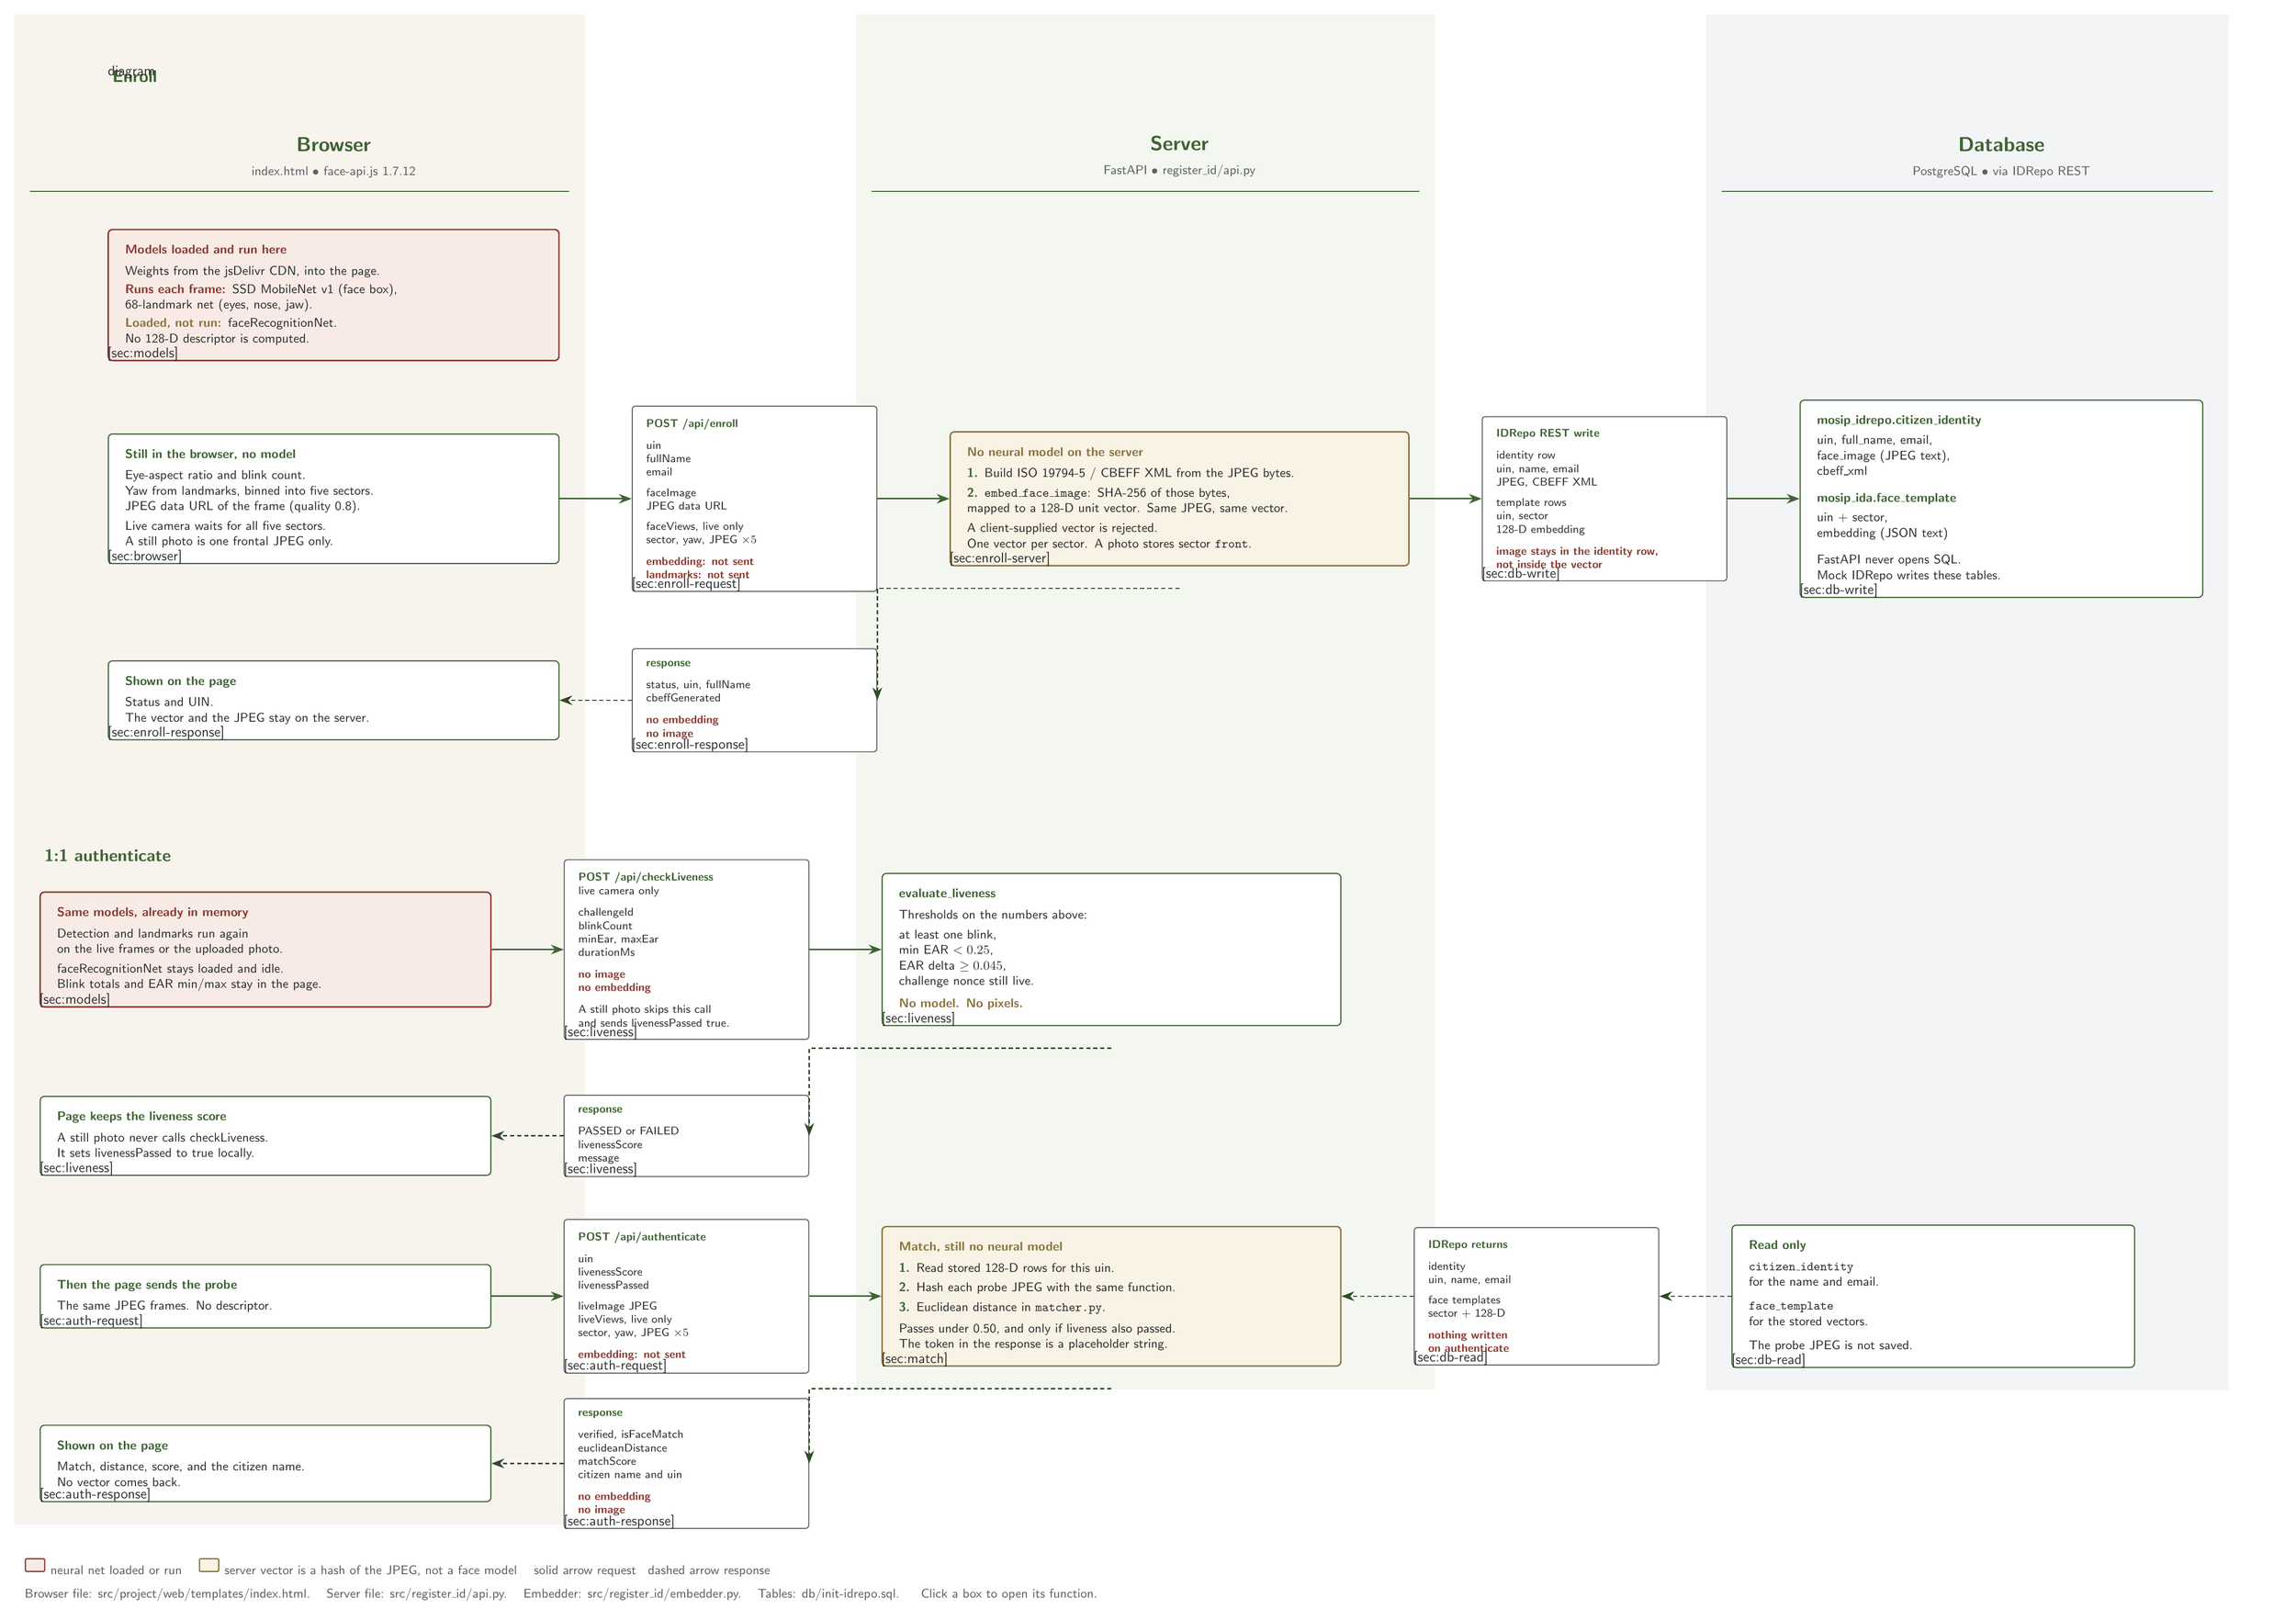
\begin{tikzpicture}[
  remember picture,
  baseline=(diagramtop),
  font=\sffamily,
  node distance=1.7cm and 1.8cm,
  every node/.style={text=ink},
  head/.style={font=\sffamily\bfseries\Large, text=green, align=center},
  sub/.style={font=\sffamily\small, text=muted, align=center},
  band/.style={font=\sffamily\bfseries\large, text=green, align=left},
  card/.style={
    draw=green, line width=0.8pt, rounded corners=3pt,
    fill=card, align=left, inner sep=12pt, inner ysep=11pt,
    font=\sffamily\small, text=ink,
    execute at begin node={\hyphenpenalty=10000\exhyphenpenalty=10000\raggedright}
  },
  model/.style={card, draw=modelstroke, line width=1.05pt, fill=modelfill},
  hash/.style={card, draw=hashstroke, line width=1pt, fill=hashfill},
  wire/.style={
    draw=muted, line width=0.7pt, rounded corners=2pt,
    fill=card, align=left, inner sep=10pt, inner ysep=9pt,
    font=\sffamily\footnotesize, text=ink,
    execute at begin node={\hyphenpenalty=10000\exhyphenpenalty=10000\raggedright}
  },
  arr/.style={
    -{Stealth[length=3.2mm,width=2.4mm]},
    draw=green, line width=1.05pt
  },
  back/.style={
    -{Stealth[length=3.2mm,width=2.4mm]},
    draw=green!75!black, line width=0.95pt, densely dashed
  },
]

% ---------- Enroll ----------
\node[band, anchor=west] (enrollband) at (0,0) {Enroll};

\node[model, text width=10.4cm, below=3.8cm of enrollband.west, anchor=north west] (bmodel) {%
  {\mk Models loaded and run here}\\[4pt]
  Weights from the jsDelivr CDN, into the page.\\[2pt]
  {\mk Runs each frame:} SSD MobileNet v1 (face box),\\
  68-landmark net (eyes, nose, jaw).\\[2pt]
  {\hk Loaded, not run:} faceRecognitionNet.\\
  No 128-D descriptor is computed.};

\node[card, text width=10.4cm, below=1.8cm of bmodel] (bsteps) {%
  {\gk Still in the browser, no model}\\[4pt]
  Eye-aspect ratio and blink count.\\
  Yaw from landmarks, binned into five sectors.\\
  JPEG data URL of the frame (quality 0.8).\\[3pt]
  Live camera waits for all five sectors.\\
  A still photo is one frontal JPEG only.};

\node[wire, text width=5.4cm, right=1.8cm of bsteps] (ew1) {%
  {\gk POST /api/enroll}\\[6pt]
  uin\\
  fullName\\
  email\\[5pt]
  faceImage\\
  JPEG data URL\\[5pt]
  faceViews, live only\\
  sector, yaw, JPEG \(\times 5\)\\[6pt]
  {\mk embedding: not sent}\\
  {\mk landmarks: not sent}};

\node[hash, text width=10.6cm, right=1.8cm of ew1] (sserver) {%
  {\hk No neural model on the server}\\[4pt]
  {\gk 1.} Build ISO 19794-5 / CBEFF XML from the JPEG bytes.\\[3pt]
  {\gk 2.} \texttt{embed\_face\_image}: SHA-256 of those bytes,\\
  mapped to a 128-D unit vector. Same JPEG, same vector.\\[3pt]
  A client-supplied vector is rejected.\\
  One vector per sector. A photo stores sector \texttt{front}.};

\node[wire, text width=5.4cm, right=1.8cm of sserver] (ew2) {%
  {\gk IDRepo REST write}\\[6pt]
  identity row\\
  uin, name, email\\
  JPEG, CBEFF XML\\[5pt]
  template rows\\
  uin, sector\\
  128-D embedding\\[6pt]
  {\mk image stays in the identity row,}\\
  {\mk not inside the vector}};

\node[card, text width=9.2cm, right=1.8cm of ew2] (db1) {%
  {\gk mosip\_idrepo.citizen\_identity}\\[3pt]
  uin, full\_name, email,\\
  face\_image (JPEG text),\\
  cbeff\_xml\\[8pt]
  {\gk mosip\_ida.face\_template}\\[3pt]
  uin + sector,\\
  embedding (JSON text)\\[8pt]
  FastAPI never opens SQL.\\
  Mock IDRepo writes these tables.};

\node[card, text width=10.4cm, below=2.4cm of bsteps] (bret) {%
  {\gk Shown on the page}\\[4pt]
  Status and UIN.\\
  The vector and the JPEG stay on the server.};

\node[wire, text width=5.4cm, right=1.8cm of bret] (eback) {%
  {\gk response}\\[6pt]
  status, uin, fullName\\
  cbeffGenerated\\[6pt]
  {\mk no embedding}\\
  {\mk no image}};

\draw[arr] (bsteps.east) -- (ew1.west);
\draw[arr] (ew1.east) -- (sserver.west);
\draw[arr] (sserver.east) -- (ew2.west);
\draw[arr] (ew2.east) -- (db1.west);
\draw[back] (sserver.south) ++(0,-0.55) -| (eback.east);
\draw[back] (eback.west) -- (bret.east);

% ---------- Authenticate ----------
\node[band, anchor=west, below=2.6cm of bret.south west] (authband) {1:1 authenticate};

\node[model, text width=10.4cm, below=0.9cm of authband.west, anchor=north west] (amodel) {%
  {\mk Same models, already in memory}\\[4pt]
  Detection and landmarks run again\\
  on the live frames or the uploaded photo.\\[3pt]
  faceRecognitionNet stays loaded and idle.\\
  Blink totals and EAR min/max stay in the page.};

\node[wire, text width=5.4cm, right=1.8cm of amodel] (aw1) {%
  {\gk POST /api/checkLiveness}\\
  live camera only\\[6pt]
  challengeId\\
  blinkCount\\
  minEar, maxEar\\
  durationMs\\[6pt]
  {\mk no image}\\
  {\mk no embedding}\\[6pt]
  A still photo skips this call\\
  and sends livenessPassed true.};

\node[card, text width=10.6cm, right=1.8cm of aw1] (alive) {%
  {\gk evaluate\_liveness}\\[4pt]
  Thresholds on the numbers above:\\[3pt]
  at least one blink,\\
  min EAR \(< 0.25\),\\
  EAR delta \(\geq 0.045\),\\
  challenge nonce still live.\\[5pt]
  {\hk No model. No pixels.}};

\node[card, text width=10.4cm, below=2.2cm of amodel] (ascore) {%
  {\gk Page keeps the liveness score}\\[4pt]
  A still photo never calls checkLiveness.\\
  It sets livenessPassed to true locally.};

\node[wire, text width=5.4cm, right=1.8cm of ascore] (aw1b) {%
  {\gk response}\\[6pt]
  PASSED or FAILED\\
  livenessScore\\
  message};

\node[card, text width=10.4cm, below=2.2cm of ascore] (asend) {%
  {\gk Then the page sends the probe}\\[4pt]
  The same JPEG frames. No descriptor.};

\node[wire, text width=5.4cm, right=1.8cm of asend] (aw2) {%
  {\gk POST /api/authenticate}\\[6pt]
  uin\\
  livenessScore\\
  livenessPassed\\[5pt]
  liveImage JPEG\\
  liveViews, live only\\
  sector, yaw, JPEG \(\times 5\)\\[6pt]
  {\mk embedding: not sent}};

\node[hash, text width=10.6cm, right=1.8cm of aw2] (amatch) {%
  {\hk Match, still no neural model}\\[4pt]
  {\gk 1.} Read stored 128-D rows for this uin.\\[3pt]
  {\gk 2.} Hash each probe JPEG with the same function.\\[3pt]
  {\gk 3.} Euclidean distance in \texttt{matcher.py}.\\[4pt]
  Passes under 0.50, and only if liveness also passed.\\
  The token in the response is a placeholder string.};

\node[wire, text width=5.4cm, right=1.8cm of amatch] (aw3) {%
  {\gk IDRepo returns}\\[6pt]
  identity\\
  uin, name, email\\[5pt]
  face templates\\
  sector + 128-D\\[6pt]
  {\mk nothing written}\\
  {\mk on authenticate}};

\node[card, text width=9.2cm, right=1.8cm of aw3] (db2) {%
  {\gk Read only}\\[4pt]
  \texttt{citizen\_identity}\\
  for the name and email.\\[6pt]
  \texttt{face\_template}\\
  for the stored vectors.\\[6pt]
  The probe JPEG is not saved.};

\node[card, text width=10.4cm, below=2.4cm of asend] (aresult) {%
  {\gk Shown on the page}\\[4pt]
  Match, distance, score, and the citizen name.\\
  No vector comes back.};

\node[wire, text width=5.4cm, right=1.8cm of aresult] (aback) {%
  {\gk response}\\[6pt]
  verified, isFaceMatch\\
  euclideanDistance\\
  matchScore\\
  citizen name and uin\\[6pt]
  {\mk no embedding}\\
  {\mk no image}};

\draw[arr] (amodel.east) -- (aw1.west);
\draw[arr] (aw1.east) -- (alive.west);
\draw[back] (alive.south) ++(0,-0.55) -| (aw1b.east);
\draw[back] (aw1b.west) -- (ascore.east);

\draw[arr] (asend.east) -- (aw2.west);
\draw[arr] (aw2.east) -- (amatch.west);
\draw[back] (db2.west) -- (aw3.east);
\draw[back] (aw3.west) -- (amatch.east);
\draw[back] (amatch.south) ++(0,-0.55) -| (aback.east);
\draw[back] (aback.west) -- (aresult.east);

% ---------- Column wells, headers, legend ----------
\coordinate (heady) at ($(bmodel.north)+(0,1.15)$);
\node[align=center, anchor=south] (bhead) at (bmodel.center |- heady) {%
  {\sffamily\bfseries\Large\color{green} Browser}\\[5pt]
  {\sffamily\small\color{muted} index.html \textbullet\ face-api.js 1.7.12}};
\node[align=center, anchor=south] (shead) at (sserver.center |- heady) {%
  {\sffamily\bfseries\Large\color{green} Server}\\[5pt]
  {\sffamily\small\color{muted} FastAPI \textbullet\ register\_id/api.py}};
\node[align=center, anchor=south] (dhead) at (db1.center |- heady) {%
  {\sffamily\bfseries\Large\color{green} Database}\\[5pt]
  {\sffamily\small\color{muted} PostgreSQL \textbullet\ via IDRepo REST}};

\coordinate (coltop) at ($(enrollband.north)+(0,0.7)$);
\node[inner sep=0pt, minimum size=1pt] (bpad) at (bmodel.center |- coltop) {};
\node[inner sep=0pt, minimum size=1pt] (spad) at (sserver.center |- coltop) {};
\node[inner sep=0pt, minimum size=1pt] (dpad) at (db1.center |- coltop) {};

\begin{scope}[on background layer]
  \node[fill=browserbg, inner xsep=18pt, inner ysep=16pt, fit=(bpad)(bmodel)(bsteps)(bret)(amodel)(ascore)(asend)(aresult)] (bwell) {};
  \node[fill=serverbg, inner xsep=18pt, inner ysep=16pt, fit=(spad)(sserver)(alive)(amatch)] (swell) {};
  \node[fill=dbbg, inner xsep=18pt, inner ysep=16pt, fit=(dpad)(db1)(db2)] (dwell) {};
\end{scope}

\draw[green, line width=0.7pt] ($(bwell.west |- heady)+(0.4,-0.22)$) -- ($(bwell.east |- heady)+(-0.4,-0.22)$);
\draw[green, line width=0.7pt] ($(swell.west |- heady)+(0.4,-0.22)$) -- ($(swell.east |- heady)+(-0.4,-0.22)$);
\draw[green, line width=0.7pt] ($(dwell.west |- heady)+(0.4,-0.22)$) -- ($(dwell.east |- heady)+(-0.4,-0.22)$);

\node[anchor=north west, font=\sffamily\small, text=muted] at ($(bwell.south west)+(0.15,-0.7)$) {%
  \tikz[baseline=-0.55ex]\draw[modelstroke, fill=modelfill, line width=0.9pt, rounded corners=1pt] (0,0) rectangle (0.48,0.32);%
  \hspace{0.4em}neural net loaded or run%
  \hspace{1.3em}%
  \tikz[baseline=-0.55ex]\draw[hashstroke, fill=hashfill, line width=0.9pt, rounded corners=1pt] (0,0) rectangle (0.48,0.32);%
  \hspace{0.4em}server vector is a hash of the JPEG, not a face model%
  \hspace{1.3em}solid arrow\ request%
  \hspace{0.9em}dashed arrow\ response};

\node[anchor=north west, font=\sffamily\small, text=muted] at ($(bwell.south west)+(0.15,-1.45)$) {%
  Browser file: src/project/web/templates/index.html.
  \hspace{0.8em}Server file: src/register\_id/api.py.
  \hspace{0.8em}Embedder: src/register\_id/embedder.py.
  \hspace{0.8em}Tables: db/init-idrepo.sql.
  \hspace{1.2em}Click a box to open its function.};

\placelink{bmodel}{sec:models}
\placelink{amodel}{sec:models}
\placelink{bsteps}{sec:browser}
\placelink{ew1}{sec:enroll-request}
\placelink{sserver}{sec:enroll-server}
\placelink{ew2}{sec:db-write}
\placelink{db1}{sec:db-write}
\placelink{eback}{sec:enroll-response}
\placelink{bret}{sec:enroll-response}
\placelink{aw1}{sec:liveness}
\placelink{alive}{sec:liveness}
\placelink{aw1b}{sec:liveness}
\placelink{ascore}{sec:liveness}
\placelink{asend}{sec:auth-request}
\placelink{aw2}{sec:auth-request}
\placelink{amatch}{sec:match}
\placelink{aw3}{sec:db-read}
\placelink{db2}{sec:db-read}
\placelink{aback}{sec:auth-response}
\placelink{aresult}{sec:auth-response}
\node[inner sep=0pt, anchor=north west] at (enrollband.north west) {\hypertarget{diagram}{}};
\coordinate (diagramtop) at (current bounding box.north);

\end{tikzpicture}

% Functions linked from the diagram. Input by current-system.tex.
\clearpage
\pagewidth=420mm
\pageheight=297mm
\setlength{\oddsidemargin}{\dimexpr12mm-1in\relax}
\setlength{\evensidemargin}{\dimexpr12mm-1in\relax}
\setlength{\topmargin}{\dimexpr12mm-1in\relax}
\setlength{\headheight}{0pt}
\setlength{\headsep}{0pt}
\setlength{\textwidth}{\dimexpr\pagewidth-24mm\relax}
\setlength{\textheight}{\dimexpr\pageheight-24mm\relax}
\setlength{\hsize}{\textwidth}
\setlength{\linewidth}{\textwidth}
\setlength{\columnwidth}{\textwidth}
\pagestyle{plain}
\sloppy
\setlength{\emergencystretch}{2em}
\lstset{%
  basicstyle=\ttfamily\footnotesize,
  breaklines=true,
  breakatwhitespace=false,
  columns=fullflexible,
  keepspaces=true,
  showstringspaces=false,
  numbers=left,
  numberstyle=\tiny\color{muted},
  numbersep=10pt,
  frame=leftline,
  framerule=1.2pt,
  rulecolor=\color{green},
  xleftmargin=2.2em,
  framesep=5pt,
  aboveskip=6pt,
  belowskip=10pt,
  tabsize=4,
  upquote=true,
  literate=
    {—}{{---}}3
    {–}{{--}}2
    {·}{{.}}1
    {…}{{...}}3
    {🎉}{{ }}1
    {❌}{{X}}1
}

\newcommand{\snippet}[3]{%
  \par
  {\sffamily\footnotesize\color{muted}\detokenize{#1}, lines #2--#3}\par
  \lstinputlisting[firstline=#2, lastline=#3, firstnumber=#2]{#1}%
}
\newcommand{\back}{\par{\sffamily\small\hyperlink{diagram}{Back to the diagram}}\par\vspace{0.4em}}

{\sffamily\bfseries\Large\color{green} Functions behind the diagram}\par
\vspace{0.4em}
{\sffamily\small The line numbers are the line numbers in the source files.
Click a box on the first page to land on its section.
Where the running code has moved on from the label in the box, the note under the heading says what the function does now.}

\section{Browser models}
\label{sec:models}
\back
{\sffamily\small\color{ink}SSD MobileNet v1 and the 68-landmark net are loaded in the page and run on each frame.
faceRecognitionNet is loaded in the same call and is not used: \texttt{analyzeSource} asks only for a box and landmarks.}

\snippet{../../src/project/web/templates/index.html}{605}{638}
\snippet{../../src/project/web/templates/index.html}{891}{910}

\clearpage
\section{Browser measurements and JPEG frames}
\label{sec:browser}
\back
{\sffamily\small\color{ink}Eye-aspect ratio, yaw, and the five sector bins are computed in the page from the landmarks.
\texttt{commitSector} stores a JPEG data URL. \texttt{viewsPayload} is what later gets posted. No embedding is built here.}

\snippet{../../src/project/web/templates/index.html}{392}{399}
\snippet{../../src/project/web/templates/index.html}{427}{433}
\snippet{../../src/project/web/templates/index.html}{483}{542}
\snippet{../../src/project/web/templates/index.html}{655}{661}

\clearpage
\section{Enroll request}
\label{sec:enroll-request}
\back
{\sffamily\small\color{ink}\texttt{captureAndEnroll} posts the UIN, name, email, and JPEG data URLs.
A live camera also sends \texttt{faceViews}. The body has no embedding field.}

\snippet{../../src/project/web/templates/index.html}{1168}{1206}

\clearpage
\section{Server enroll}
\label{sec:enroll-server}
\back
{\sffamily\small\color{ink}\texttt{enroll\_citizen\_endpoint} builds the CBEFF XML, then hashes each JPEG.
\texttt{embed\_face\_image} is that hash. It is not a face model.
\texttt{\_templates\_for\_enrollment} refuses to trust a vector that arrived from the browser.}

\snippet{../../src/register_id/api.py}{38}{73}
\snippet{../../src/register_id/api.py}{146}{191}
\snippet{../../src/register_id/embedder.py}{15}{44}

\clearpage
\section{Database write}
\label{sec:db-write}
\back
{\sffamily\small\color{ink}The gateway posts to IDRepo. The mock service writes the JPEG and CBEFF onto \texttt{citizen\_identity}, and the 128-D vectors onto \texttt{face\_template}. FastAPI does not open SQL.}

\snippet{../../src/register_id/idrepo_client.py}{154}{241}
\snippet{../../src/mock/idrepo/storage.py}{173}{267}
\snippet{../../db/init-idrepo.sql}{1}{29}

\clearpage
\section{Enroll response}
\label{sec:enroll-response}
\back
{\sffamily\small\color{ink}The endpoint returns status, UIN, and name. The vector and the JPEG are not in that JSON.}

\snippet{../../src/register_id/api.py}{183}{190}

\clearpage
\section{Liveness numbers}
\label{sec:liveness}
\back
{\sffamily\small\color{ink}\texttt{evaluate\_liveness} is still the body of \texttt{POST /api/checkLiveness}: blink count and eye-aspect thresholds, no pixels.
On the authenticate path the page does not call that route. Opening the camera posts \texttt{/api/sweep/challenge} instead, and the later authenticate body sends \texttt{livenessPassed: false}.}

\snippet{../../src/register_id/api.py}{139}{144}
\snippet{../../src/register_id/liveness.py}{54}{106}
\snippet{../../src/project/web/templates/index.html}{581}{601}
\snippet{../../src/register_id/api.py}{94}{99}
\snippet{../../src/register_id/sweep.py}{42}{63}

\clearpage
\section{Authenticate request}
\label{sec:auth-request}
\back
{\sffamily\small\color{ink}The page posts the UIN, the sweep challenge id, and the five JPEG views.
\texttt{livenessScore} is 0 and \texttt{livenessPassed} is false. No embedding is sent.}

\snippet{../../src/project/web/templates/index.html}{1290}{1328}

\clearpage
\section{Server check of the five images}
\label{sec:match}
\back
{\sffamily\small\color{ink}\texttt{POST /api/authenticate} calls \texttt{assess\_sweep}.
That check hashes each JPEG only to reject a repeated picture, and it checks that the client yaw labels run left to right.
It does not compare the probe with the stored gallery, and it does not treat the result as a face match. \texttt{isFaceMatch} is returned false.}

\snippet{../../src/register_id/api.py}{219}{254}
\snippet{../../src/register_id/sweep.py}{31}{39}
\snippet{../../src/register_id/sweep.py}{90}{162}
\snippet{../../src/register_id/matcher.py}{11}{54}

\clearpage
\section{Database read}
\label{sec:db-read}
\back
{\sffamily\small\color{ink}Authenticate loads the identity row so the response can name the citizen.
\texttt{get\_face\_templates} is the read of the stored vectors. The authenticate endpoint above does not call it.}

\snippet{../../src/register_id/idrepo_client.py}{243}{265}
\snippet{../../src/register_id/idrepo_client.py}{267}{290}
\snippet{../../src/mock/idrepo/storage.py}{279}{308}

\clearpage
\section{Authenticate response}
\label{sec:auth-response}
\back
{\sffamily\small\color{ink}The page shows the sweep message. The JSON still carries distance and score fields; the endpoint fills distance with 1 and the score with 0, and it does not return an embedding or an image.}

\snippet{../../src/register_id/api.py}{236}{254}
\snippet{../../src/project/web/templates/index.html}{1329}{1370}

\end{document}
